%!TEX root = ../main.tex

\section{Differential cross section}
\label{sec:differential-cross-section}

As a second task, the validity of the Klein-Nishina formula presented in
\autoref{eq:klein-nishina-cross-section} is tested. For this purpose, the
spectrometer is placed at various angles relative to the beam path. For every angle
two measurements of \SI{300}{\second} each are taken. One measurement with a
cylindrical aluminum target in the beam path that allows for compoton scattering.
The second measurement is conducted without any target and will help quantify the
background noise measured by the spectrometer. The resulting distribution of
electron energies is shown in \autoref{fig:diff-measurements} for all measurements.

\begin{figure}
  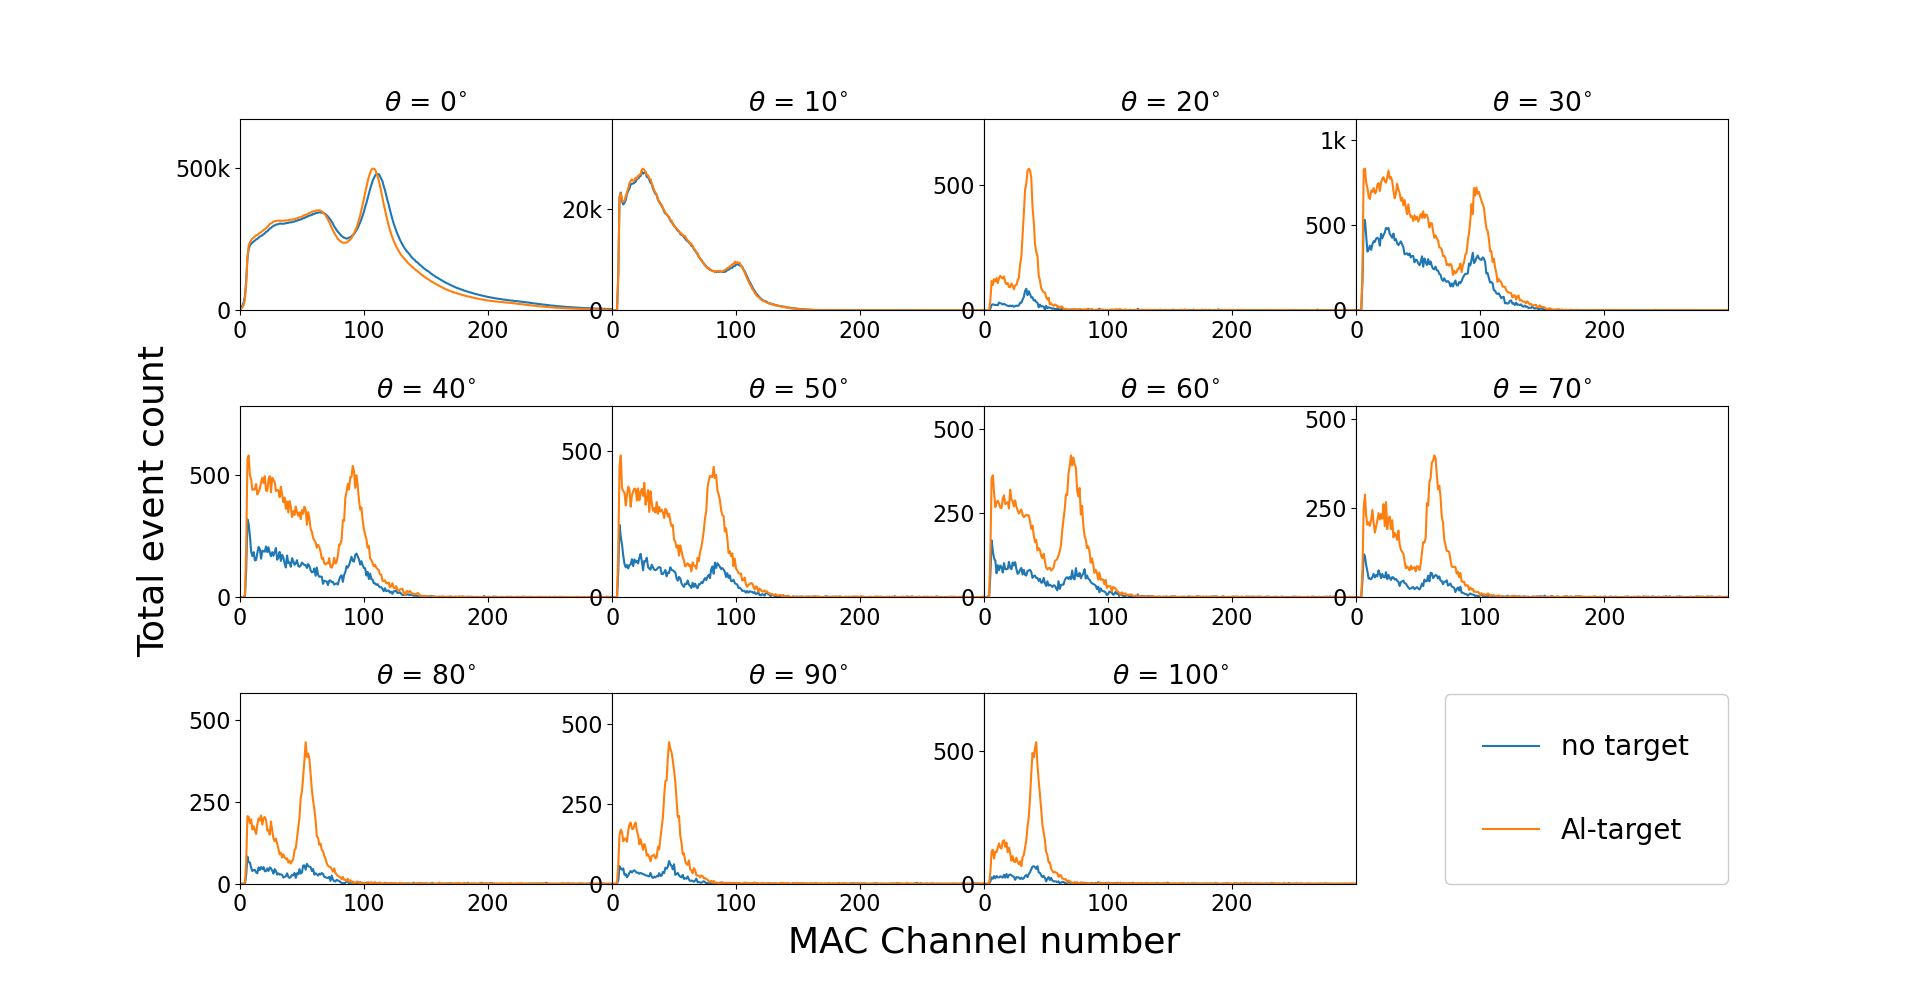
\includegraphics[width=1.0\textwidth]{./fig/differential measurements.png}
  \caption{}{Raw number of events counted in every channel for each measured angle.
  The dashed black lines indicate the theoretical energy a photon has after
  undergoing compton scattering at an angle $\theta$. The distance between signal
  peaks and this energy grows with increasing scattering angles. This is expected
  due to the imperfect calibration.}\label{fig:diff-measurements}
\end{figure}
